\documentclass[aspectratio=169, 11pt, hyperref={unicode}]{beamer}
\usetheme{Madrid}
\usepackage{pgfplots}
\pgfplotsset{compat=1.17}

\usepackage[british]{babel}
\usepackage[utf8]{inputenc}
\usepackage[T1]{fontenc}

\usepackage[nodayofweek]{datetime}
\newdate{Date}{26}{1}{2024}

\usepackage{graphicx}
\usepackage{subcaption}
\usepackage{hyperref}
\hypersetup{colorlinks=false}

\usepackage[euler]{textgreek}
\usepackage[font=footnotesize]{caption}


\title{VGA Brownian motion}
\subtitle{B2M34NSV -- Semester project}
\author{Martin Šimák}
\date{\displaydate{Date}}


\definecolor{cvut_navy}{HTML}{0065BD}
\definecolor{cvut_blue}{HTML}{6AADE4}
\definecolor{cvut_gray}{HTML}{156570}

\setbeamercolor{section in toc}{fg=black,bg=white}
\setbeamercolor{alerted text}{fg=cvut_blue}
\setbeamercolor*{palette primary}{bg=cvut_navy,fg=gray!20!white}
\setbeamercolor*{palette secondary}{bg=cvut_blue,fg=white}
\setbeamercolor*{palette tertiary}{parent=palette primary}
\setbeamercolor*{palette quaternary}{fg=green,bg=gray!5!white}

\setbeamercolor*{sidebar}{fg=cvut_navy,bg=gray!15!white}


\setbeamercolor{titlelike}{parent=palette primary}
\setbeamercolor{frametitle}{parent=palette primary}

\setbeamercolor*{separation line}{}
\setbeamercolor*{fine separation line}{}

\setbeamertemplate{navigation symbols}{} 

\setbeamercolor{itemize item}{fg=cvut_blue}
\setbeamercolor{itemize subitem}{fg=cvut_blue}
\setbeamercolor{itemize subsubitem}{fg=cvut_blue}
\setbeamercolor{section number projected}{bg=cvut_navy}
\setbeamercolor{caption name}{fg=cvut_blue}

\setbeamertemplate{itemize item}[circle]
\setbeamertemplate{itemize subitem}[circle]
\setbeamertemplate{itemize subsubitem}[circle]
\setbeamertemplate{caption}[numbered]

\def\MHz{\,\mathrm{MHz}}
\def\Hz{\,\mathrm{Hz}}


\begin{document}

\logo{
\includegraphics[height=1cm]{src/symbol_cvut_plna_samostatna_verze.pdf}}

\begin{frame}
	\titlepage
\end{frame}

\begin{frame}
    \frametitle{Contents}
    \tableofcontents
\end{frame}

\section{Task introduction}
\begin{frame}{Task introduction}
\begin{itemize}
    \item \emph{Task:} Brownian motion of molecules displayed using a VGA interface.
    \item \emph{Development board:} Digilent Basys 3 featuring the Xilinx Artix-7 FPGA.
\end{itemize}
\end{frame}


\section{Modules}
\begin{frame}{Clock divider}
    \begin{minipage}{.45\textwidth}
        Division of system clock ($100\MHz$) into multiple clock signals:
        \begin{itemize}
            \item $50\MHz$ clock for VGA controls,
            \item $100\Hz$ clock for Ball1 movement,
            \item $50\Hz$ clock for Ball2 movement,
            \item $4\Hz$ clock for Ball1 collision generation,
            \item $4\Hz$ clock for Ball2 collision generation.
        \end{itemize}
    \end{minipage}
    ~
    \begin{minipage}{.45\textwidth}
        \begin{figure}[!ht]
            \centering
            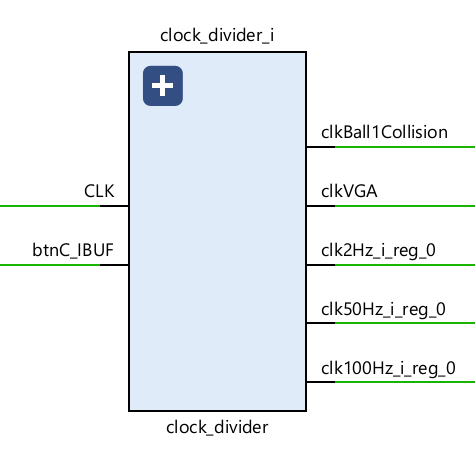
\includegraphics[width=\textwidth]{src/clock-divider.png}
        \end{figure}
    \end{minipage}
\end{frame}

\begin{frame}{Frame graphical component}
    \begin{minipage}{.45\textwidth}
        Bounding frame drawing component
        \begin{itemize}
            \item \emph{In:} Clock signal ($50\MHz$), asynchronous reset, current drawing position coordinates.
            \item \emph{Out:} RGB colour signals.
        \end{itemize}
    \end{minipage}
    ~
    \begin{minipage}{.45\textwidth}
        \begin{figure}[!ht]
            \centering
            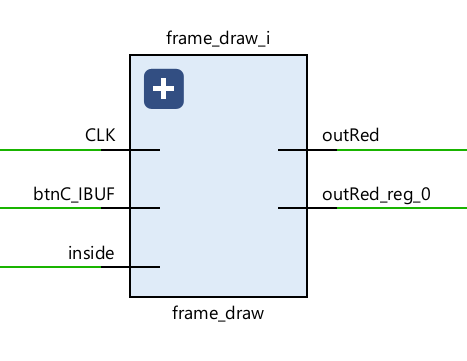
\includegraphics[width=\textwidth]{src/frame-draw.png}
        \end{figure}
    \end{minipage}
\end{frame}

\begin{frame}{LFSR}
    \begin{minipage}{.45\textwidth}
        Pseudorandom generator of virtual collisions
        \begin{itemize}
            \item \emph{In:} Clock signal ($4\Hz$ or $2\Hz$), asynchronous reset, enable bit.
            \item \emph{Out:} MSB, LSB.
        \end{itemize}
    \end{minipage}
    ~
    \begin{minipage}{.45\textwidth}
        \begin{figure}[!ht]
            \centering
            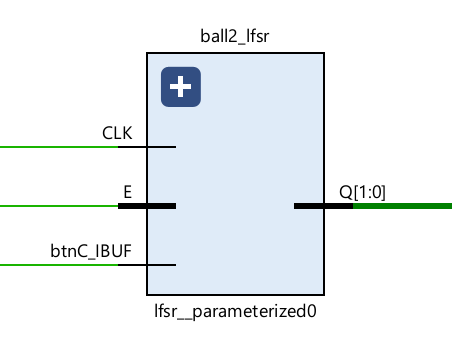
\includegraphics[width=\textwidth]{src/lfsr.png}
        \end{figure}
    \end{minipage}
\end{frame}

\begin{frame}{Ball movement control}
    \begin{minipage}{.45\textwidth}
        Ball movement controller responsible for collision detection
        \begin{itemize}
            \item \emph{In:} Clock signal ($100\Hz$ or $50\Hz$), asynchronous reset, virtual collision bits, current other ball coordinates.
            \item \emph{Out:} Current position coordinates of the drawn ball.
        \end{itemize}
    \end{minipage}
    ~
    \begin{minipage}{.45\textwidth}
        \begin{figure}[!ht]
            \centering
            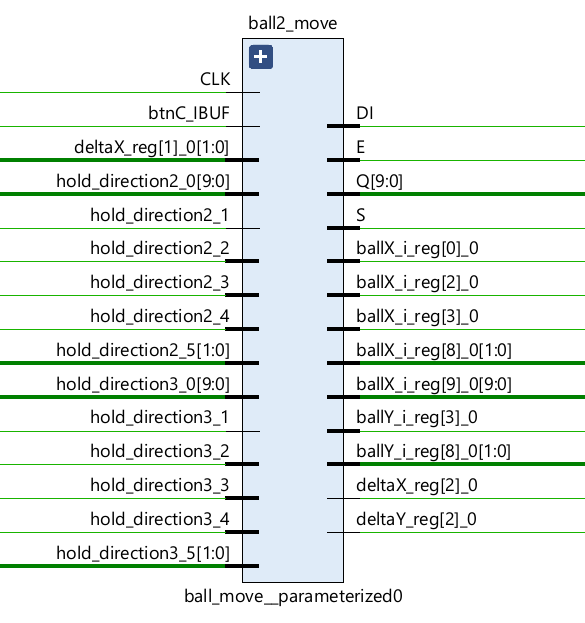
\includegraphics[width=\textwidth]{src/ball-move.png}
        \end{figure}
    \end{minipage}
\end{frame}

\begin{frame}{Ball graphical component}
    \begin{minipage}{.45\textwidth}
        Ball drawing component
        \begin{itemize}
            \item \emph{In:} Clock signal ($50\MHz$), asynchronous reset, current ball and drawing coordinates.
            \item \emph{Out:} RBG colour signals.
        \end{itemize}
    \end{minipage}
    ~
    \begin{minipage}{.45\textwidth}
        \begin{figure}[!ht]
            \centering
            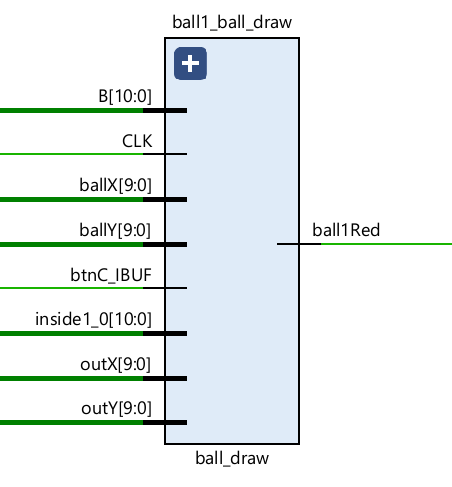
\includegraphics[width=\textwidth]{src/ball-draw.png}
        \end{figure}
    \end{minipage}
\end{frame}

\begin{frame}{Colour multiplexer}
    \begin{minipage}{.45\textwidth}
        Combiner of RBG colour signals from all present objects
        \begin{itemize}
            \item \emph{In:} Clock signal ($50\MHz$), asynchronous reset, RGB colour signals from all present objects.
            \item \emph{Out:} Combined RGB colour signals.
        \end{itemize}
    \end{minipage}
    ~
    \begin{minipage}{.45\textwidth}
        \begin{figure}[!ht]
            \centering
            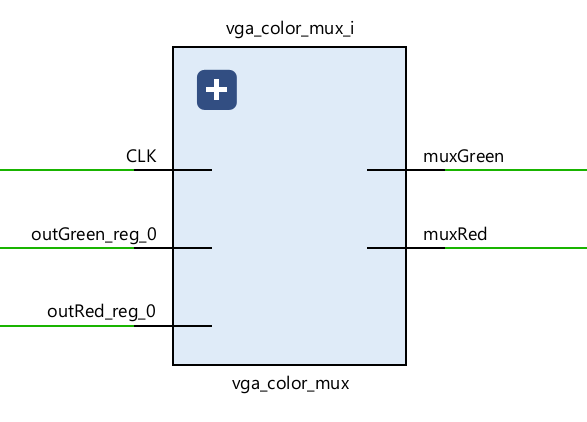
\includegraphics[width=\textwidth]{src/color-mux.png}
        \end{figure}
    \end{minipage}
\end{frame}

\begin{frame}{VGA driver}
    \begin{minipage}{.45\textwidth}
        VGA signal generator
        \begin{itemize}
            \item \emph{In:} Clock signal ($50\MHz$), asynchronous reset, RGB colour signals.
            \item \emph{Out:} Vertical and horizontal synchronization signals, VGA colour signals, current drawing coordinates.
        \end{itemize}
    \end{minipage}
    ~
    \begin{minipage}{.45\textwidth}
        \begin{figure}[!ht]
            \centering
            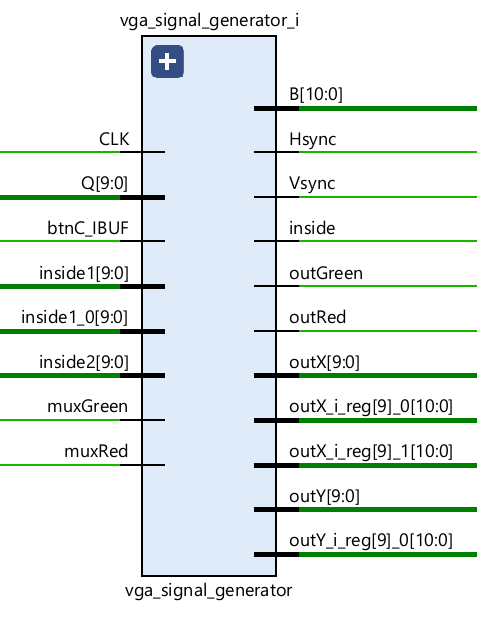
\includegraphics[scale=.5]{src/vga-signal-generator.png}
        \end{figure}
    \end{minipage}
\end{frame}

\section{Conclusion}
\begin{frame}{Conclusion}
    What has been implemented:
	\begin{itemize}
        \item two molecules moving in a pseudorandom pattern,
        \item collision detection.
    \end{itemize}
    Possible improvements:
    \begin{itemize}
        \item better collision detection resolution.
    \end{itemize}
\end{frame}

\setbeamercolor{background canvas}{bg=white}

\end{document}
